\chapter{Introduction}\label{chap:introduction}

Describe the problem and the motivation for this research.
\\
\section{Related Work}\label{sec:related_work}

Describe the current state of the art. Provide all necessary citations.



\section{MBZIRC challenge}


\begin{figure}[!htbp]
    \centering
    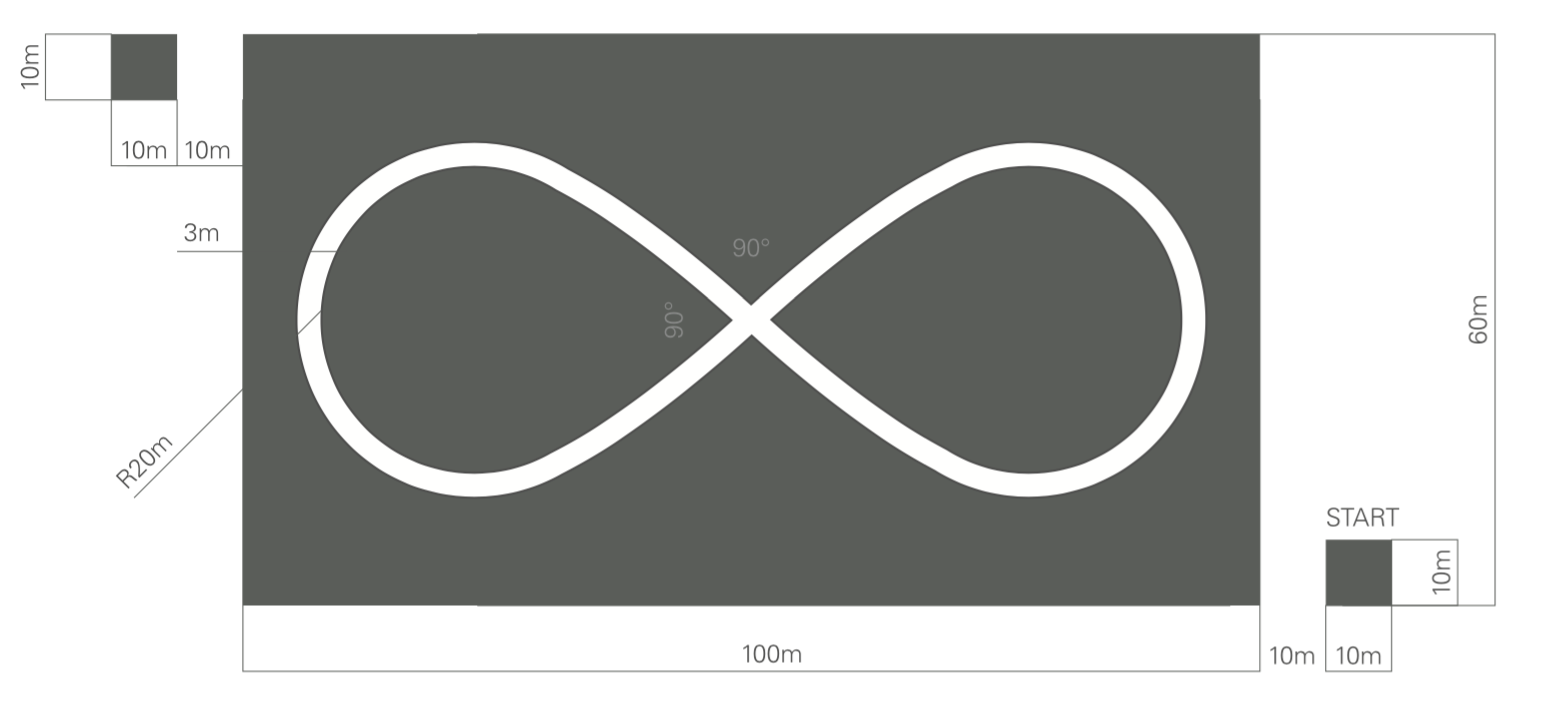
\includegraphics[width=1.1\textwidth]{img/arena.png}
    \caption{Arena of the challenge}
    \label{fig:arenachallenge}
\end{figure}

\paragraph{Design of the platform}

\paragraph{Infinity shape path}
In the MBZIRC challenge the moving platform will move in an infinity-shape path described in the figure \ref{fig:arenachallenge}. 
We need to describe in a mathematical way this shape in order to use this information in the prediction step of the EKF.
From the specification of the challenge:
\begin{itemize}
\item the car is moving with constant velocity $v$ along the path
\item the radius of the circumferences that forms the trajectory is $r_{8}$m
\item the path is making a cross in the middle that creates 4 angles of $\frac{\pi}{2}$ 
\end{itemize}
The easiest way to describe this path is to define how the angle $\theta$ is changing in function of the space. \\
It easy to see that the shape can be seen as a combination of a cross and two circles.
The cross is simply defined as the union between the two line:
\begin{align}
\begin{split}
y &= x \\
y &= -x
\end{split}
\end{align}
while the two circles 
\begin{align}
\begin{split}
y^2 + (x - x_0)^2 &= r_{8}^2 \\
y^2 + (x + x_0)^2 &= r_{8}^2 
\end{split}
\end{align}
It easy to see that if we want the intersections between these two functions to be exactly in the 4 points we have to choose 
\begin{align}
\begin{split}
x_0 = \frac{\sqrt{2}}{2}r_{8}
\end{split}
\end{align}
That correspond to the 4 intersections coordinate
\begin{align}
\begin{split}
\Big(\frac{\sqrt{2}}{2}r_{8},\frac{\sqrt{2}}{2}r_{8}\Big);
\Big(\frac{\sqrt{2}}{2}r_{8},-\frac{\sqrt{2}}{2}r_{8}\Big);
\Big(-\frac{\sqrt{2}}{2}r_{8},-\frac{\sqrt{2}}{2}r_{8}\Big);
\Big(-\frac{\sqrt{2}}{2}r_{8},\frac{\sqrt{2}}{2}r_{8}\Big)
\end{split}
\end{align}

\begin{figure}[!htbp]
  \centering
 {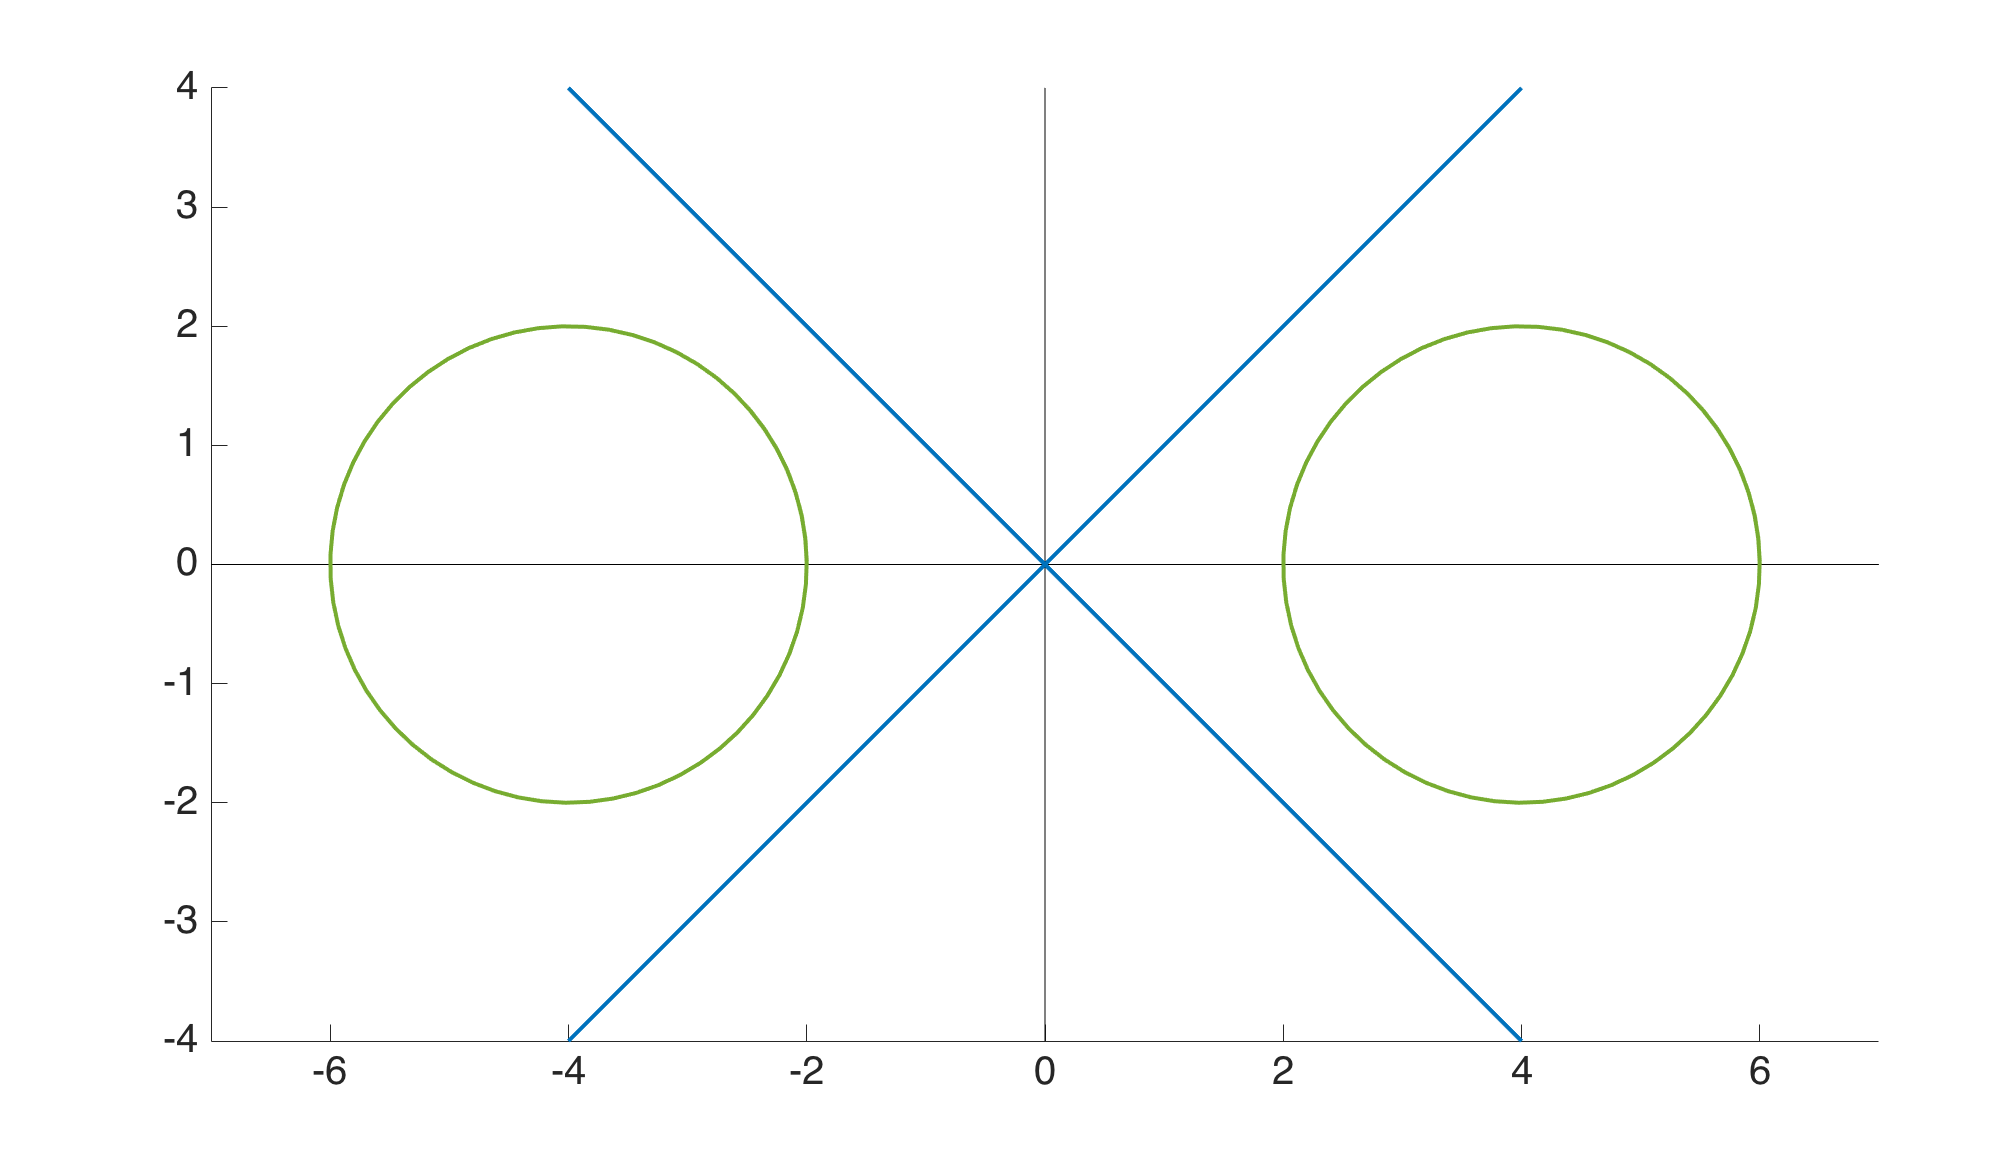
\includegraphics[width=0.48\textwidth]{img/constructionshape1_.png}\label{fig:constuctinfinity1}}
  \hfill
  {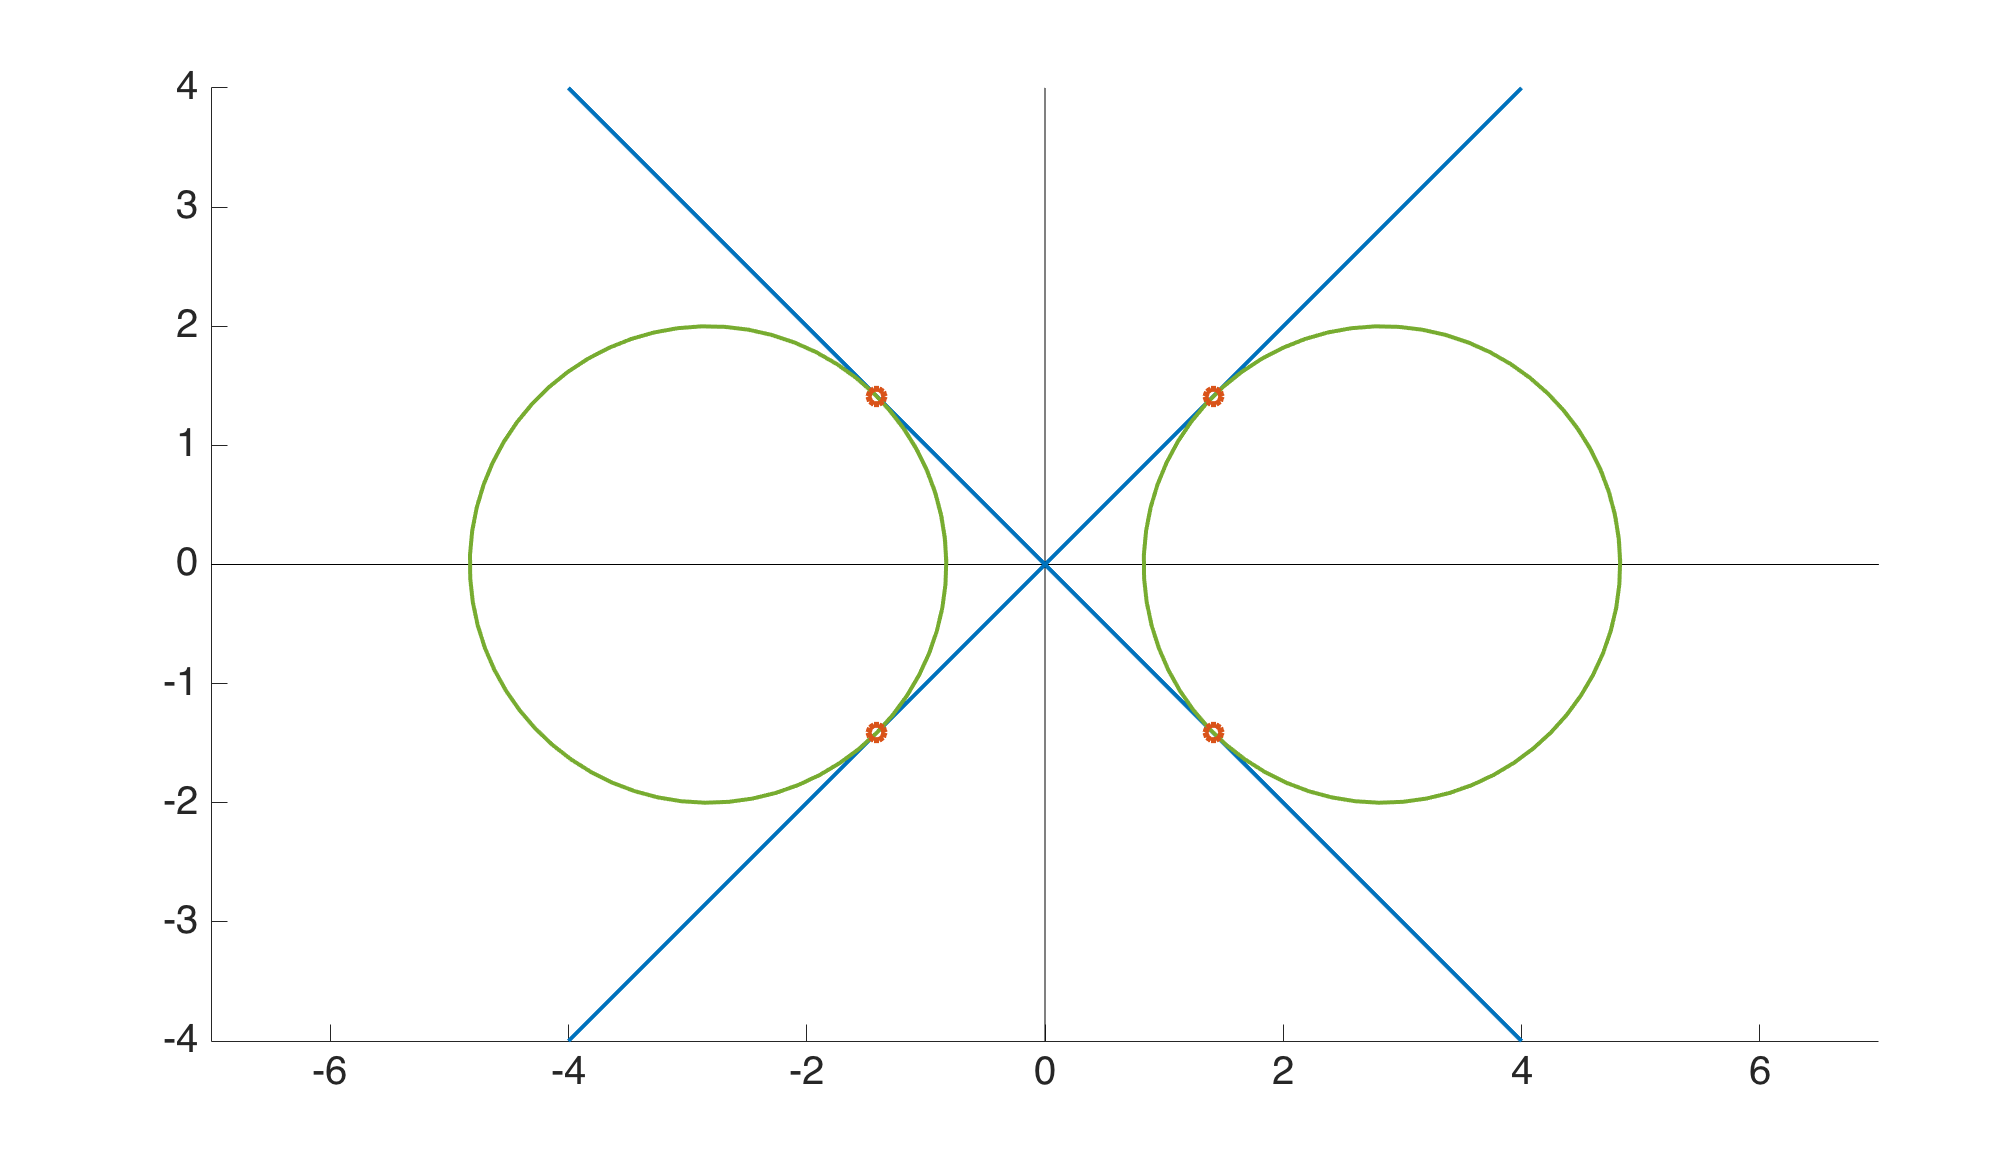
\includegraphics[width=0.48\textwidth]{img/constructionshape2_.png}\label{fig:constuctinfinity2}}
  \caption{How to construct the infinity-shape path}
\end{figure}

If we travel over the two circumferences the intersections correspond to angles $\theta = \pm \frac{3\pi}{4}$. \\
Now it is obvious to see that the path is symmetric and it can be divided in 4 parts and describing how the angle is changing in one of this section, the whole trajectory is defined.\\
We can observe that:
\begin{align}
\theta(x) =
\begin{cases}
    -\frac{x}{r_{8}}  &x\in \Big[0,\frac{3\pi}{4}r_{8}\Big] \quad \quad \ \ \  \\[10pt]
    -\frac{3\pi}{4} &x\in \Big[\frac{3\pi}{4}r_{8} ,\frac{3\pi}{4}r_{8} + r_{8}\Big]
\end{cases}
\end{align}
This function define a quarter of the trajectory \ref{fig:quarter_path} in function of the radius $r_{8}$ of the path.\\
It is now possible to use it to generate the entire trajectory $(x(t),y(t))$\ref{fig:entire_path}: we know that the length of the path is $l = 4(\frac{3\pi}{4}r_{8} + r_{8})$ and given the constant velocity $v$ we can calculate the time to complete the trajectory $T = \frac{l}{v}$ and it is simple to define $\theta(t)$ just stretching or shrinking $\theta(x)$ .\\
So we can define
\begin{align}
\begin{split}
\dot{x} &= v cos(\theta(t)) \\
\dot{y} &= v sin(\theta(t))
\end{split}
\end{align}
And finally we have
\begin{align}
\begin{split}
x_k &= x_{k-1} + dt \big(v_{k-1} cos(\theta_{k-1})\big) \\
y_k &= y_{k-1} + dt \big(v_{k-1} sin(\theta_{k-1})\big)
\end{split}
\end{align}

\begin{figure}[!htbp]
  \centering
 {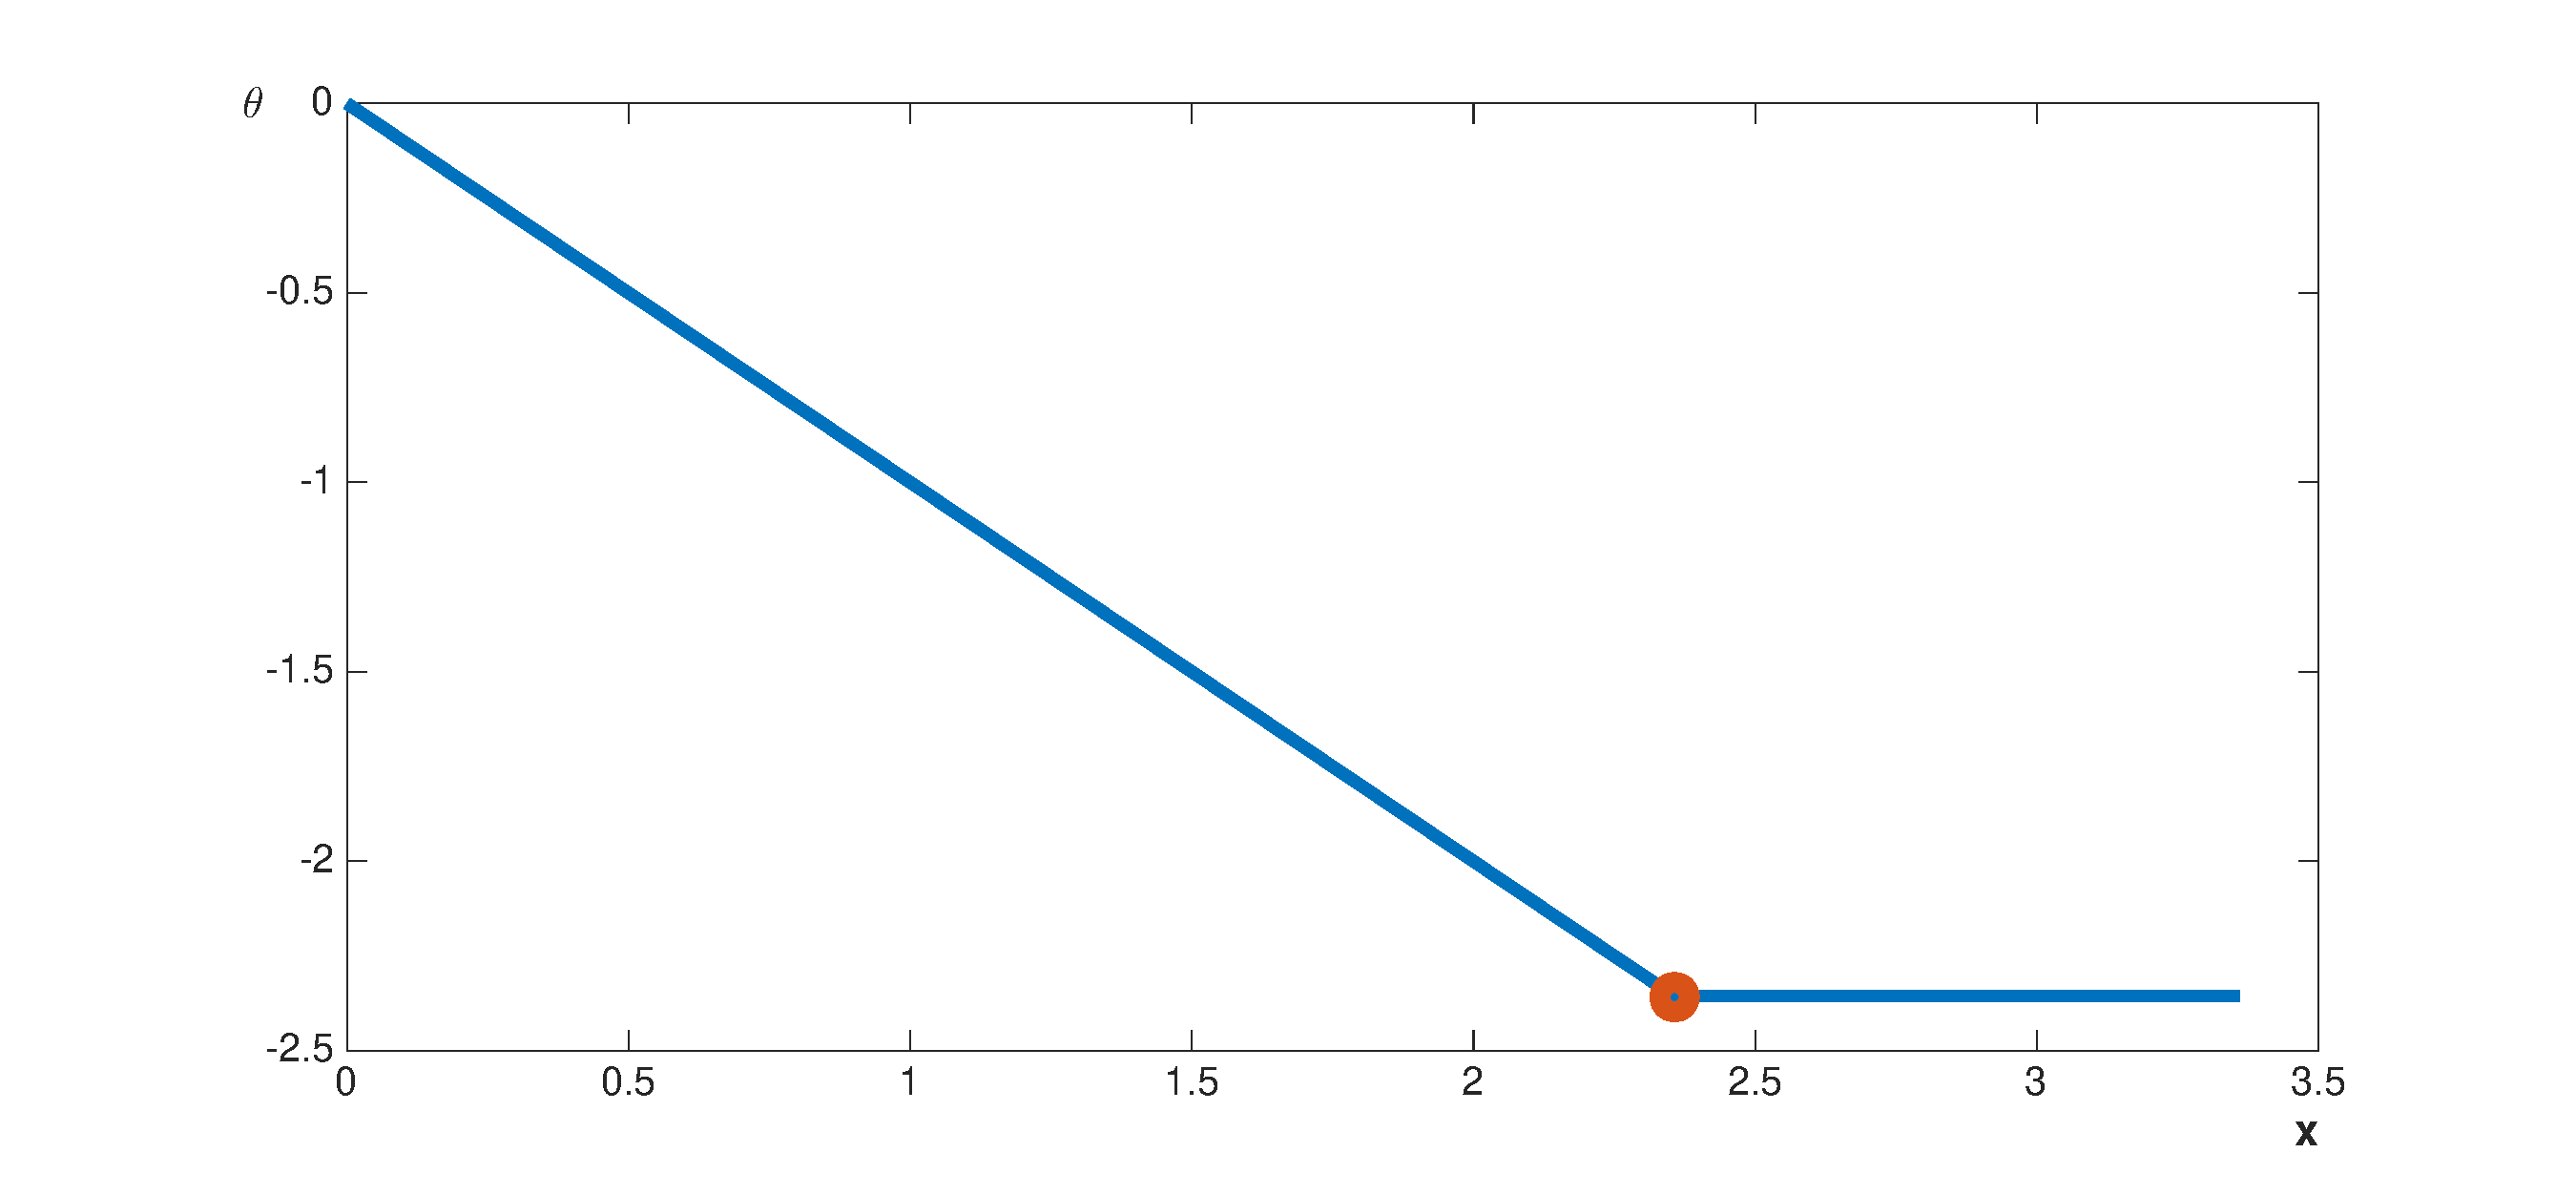
\includegraphics[width=0.8\textwidth]{img/angle_x.eps}\label{fig:quarter_theta}}
  \hfill
  {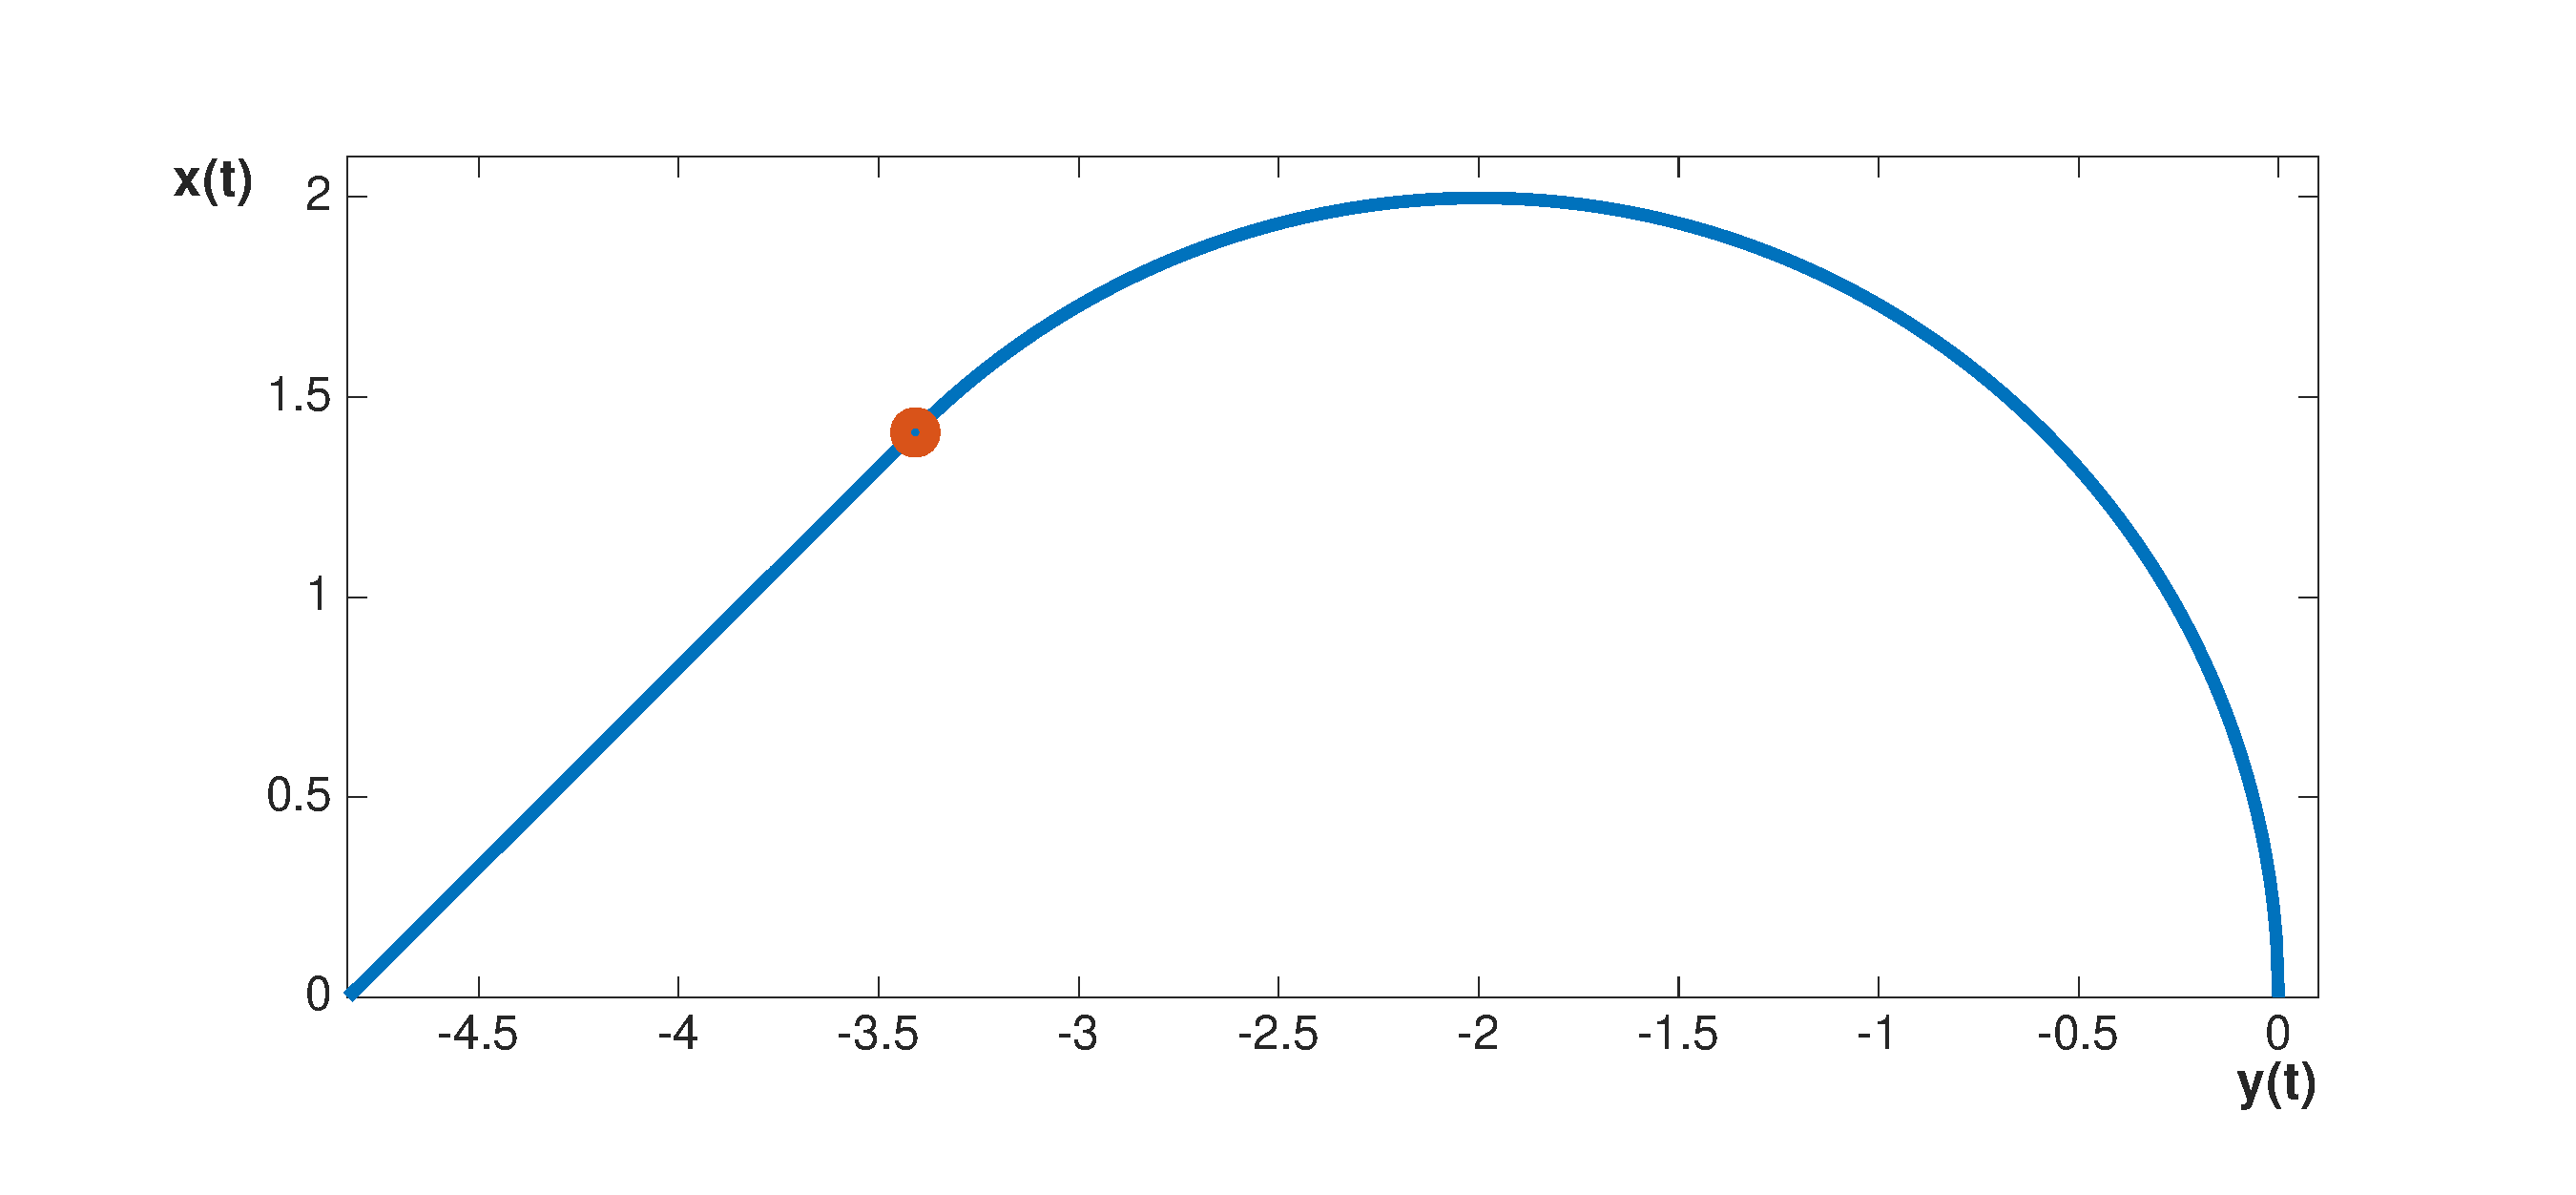
\includegraphics[width=0.8\textwidth]{img/path_x_quarter.eps}\label{fig:quarter_xy}}
  \caption{The parametrization of a quarter of the path}
  \label{fig:quarter_path}
\end{figure}

\begin{figure}[!htbp]
    \centering
    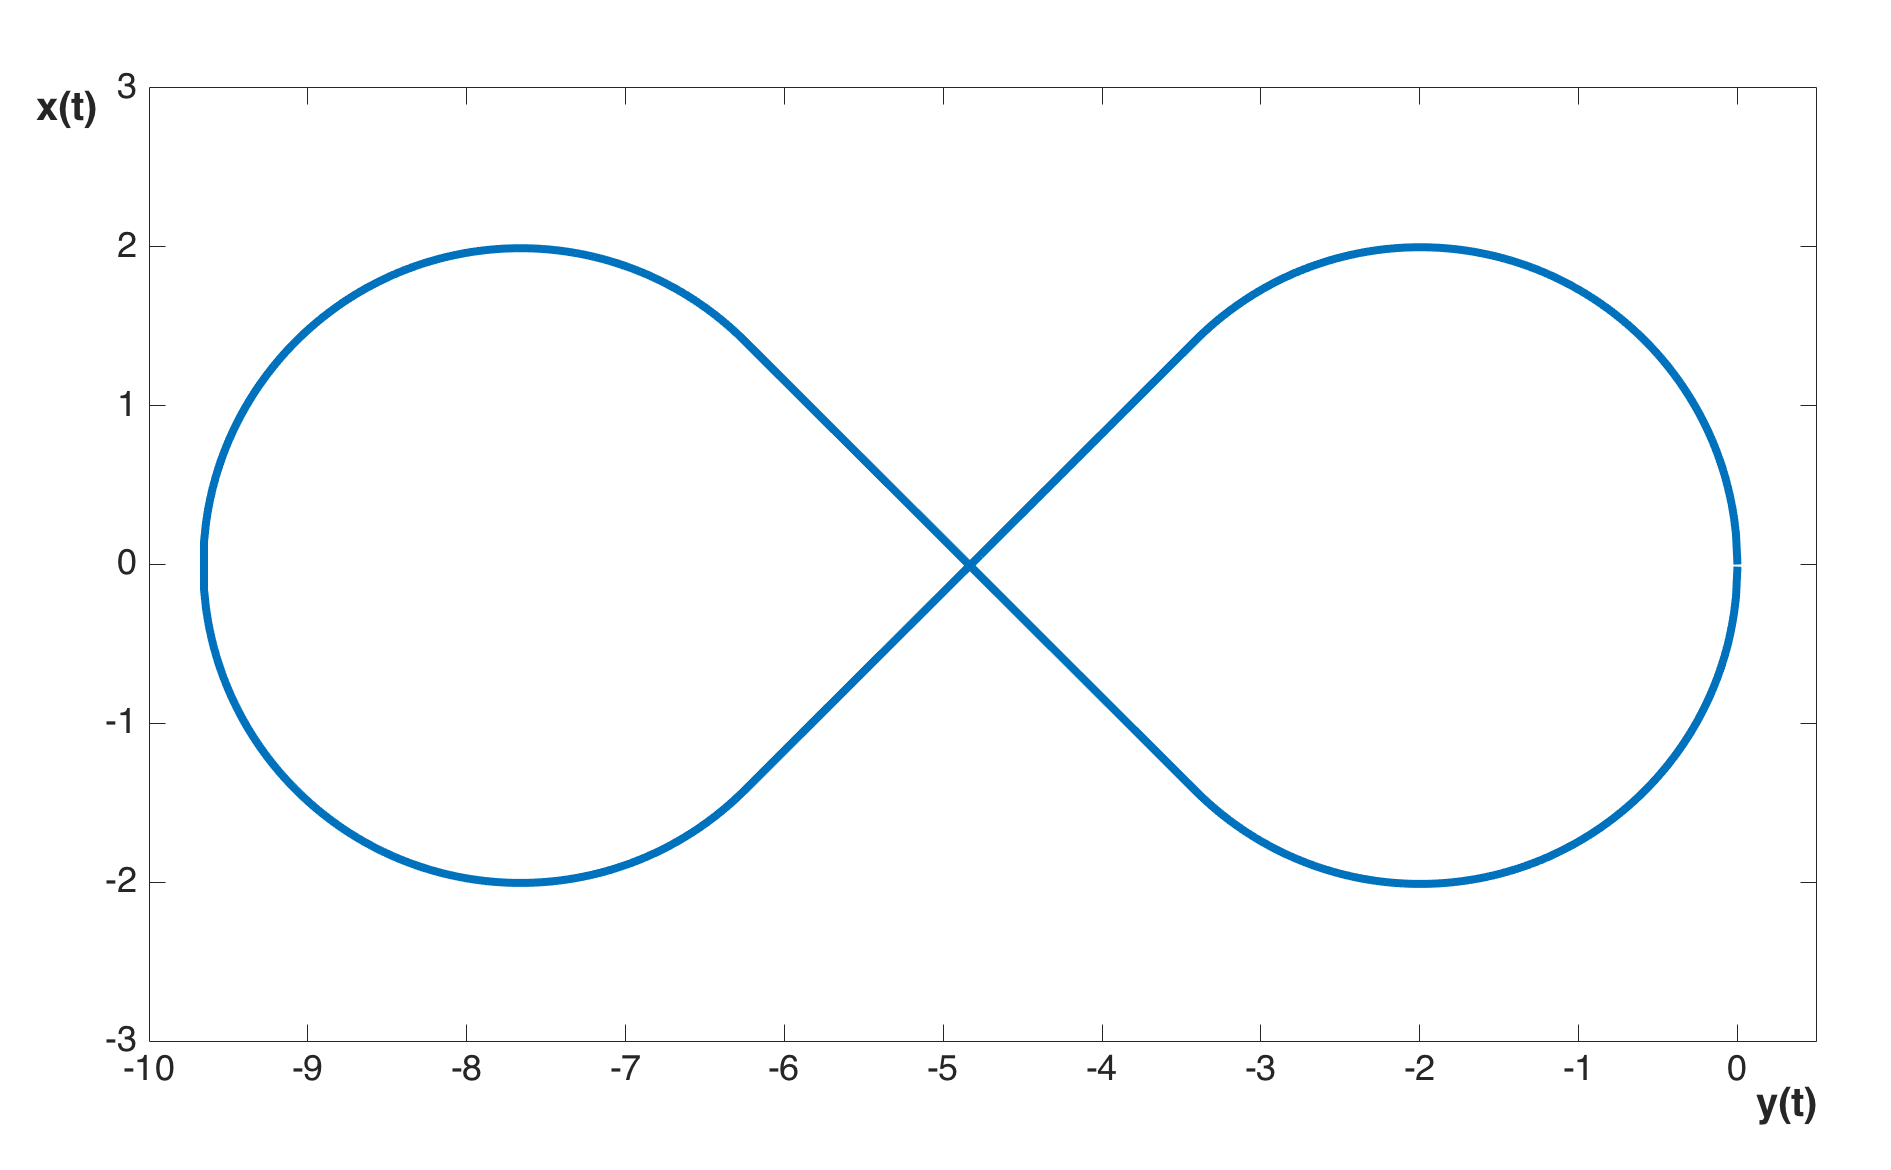
\includegraphics[width=1\textwidth]{img/infinityshapepath.png}
    \caption{Infinity-shape path}
    \label{fig:entire_path}
\end{figure}


